\begin{center}
	{\scriptsize
		\begin{tabularx}{\textwidth}{p{0.2\textwidth}|p{0.6\textwidth}|p{0.1\textwidth}}
			\caption{Summary of methods for reaching the objectives} \label{tab:methods_per_objective} \\
			\hline 
			\hline 
			\textbf{Objectives} & 
			\textbf{Methods} &
			\textbf{Locations}\\ 
			\hline 
			\endfirsthead
			\multicolumn{3}{c}%
			{\textit{Continued from previous page}} \\
			\hline
			\hline 
			\textbf{Objectives} & 
			\textbf{Methods} &
			\textbf{Locations}\\ 
			\hline 
			\endhead
			\hline 
			\multicolumn{3}{r}{\textit{Continued on next page}} \\ 
			\endfoot
			\hline 
			\endlastfoot
			\hline
			
			
			\Paste{GO} & \blindlist{enumerate} & Sec.~\ref{sec:implement} on p.~\pageref{sec:implement}\\ \hline
			
			
			\Paste{SO1} & \blindlist{enumerate} & Sec.~\ref{sec:implement} on p.~\pageref{sec:implement} \\ \hline
			
			
			\Paste{SO2} & \blindlist{enumerate} & Sec.~\ref{sec:implement} on p.~\pageref{sec:implement}\\ \hline
			
			
			\Paste{SO3} & \blindlist{enumerate} & Sec.~\ref{sec:implement} on p.~\pageref{sec:implement}\\ \hline
			
			
			\Paste{SO4} & \blindlist{enumerate} & Sec.~\ref{sec:implement} on p.~\pageref{sec:implement} \\ \hline
			
			
			\Paste{SO5} & \blindlist{enumerate} & Sec.~\ref{sec:implement} on p.~\pageref{sec:implement} \\ \hline
			
		\end{tabularx}
	}
\end{center}

\section{Research Design}
% TODO: Write content

\section{Data Collection}
\subsection{Utilization of Open-Source Databases}
% TODO: Cite Kaggle dataset
To establish a foundation for the system's model, the group initially referenced an open-source dataset from Kaggle [x]. This dataset provides an original 500x500px images of Arabica green coffee beans categorize as defective or good. This dataset also provided insights into how individual beans were captured, including factors such as lighting, camera positioning, focus, and resolution. By analyzing the dataset, the group gained a better understanding of how to achieve a high-quality data collection, ensuring that the collected dataset would contribute to high model accuracy when it is fed into the system.

\subsection{Manual Sorting}

\begin{figure}[h]
    \centering
    \includegraphics[width=6cm]{manual_sorting}
    \caption{Manual Sorting Process}
    \label{fig:manual_sorting}
\end{figure}

% TODO: Fix citations
The diagram in Figure \ref{fig:manual_sorting} depicts the representation of the process of manual sorting of unsorted green coffee beans through a series of steps. First, the beans are sorted by density using methods such as floatation or shaking tables. This helps in separating the denser beans, usually pertaining to a more developed and higher quality bean. Then, the beans are sorted by size using screens and sieves with specific dimensions depending on the variety of the beans. After this, a thorough visual inspection is performed by the sorters to identify and remove the defective beans from the batch. To ensure consistency and accuracy, the group follows the Specialty Coffee Association of America (SCAA) Standards Defect Handbook, which provide documentation and guidelines for identifying and classifying defective beans [x]. Finally, the process results in the output of sorted green coffee beans, ready for further processing or sale. 
To ensure the dataset reflects real-world conditions, the group acquired Arabica green coffee beans from Davao. These beans were manually sorted to properly classify defective characteristics before capturing images for dataset creation. This step was crucial for improving the efficiency of batch image capture and ensuring accurate model training, making the system more applicable to Philippine coffee producers.

\subsection{1st Iteration: Controlled Setup}
\begin{figure}[h]
    \centering
    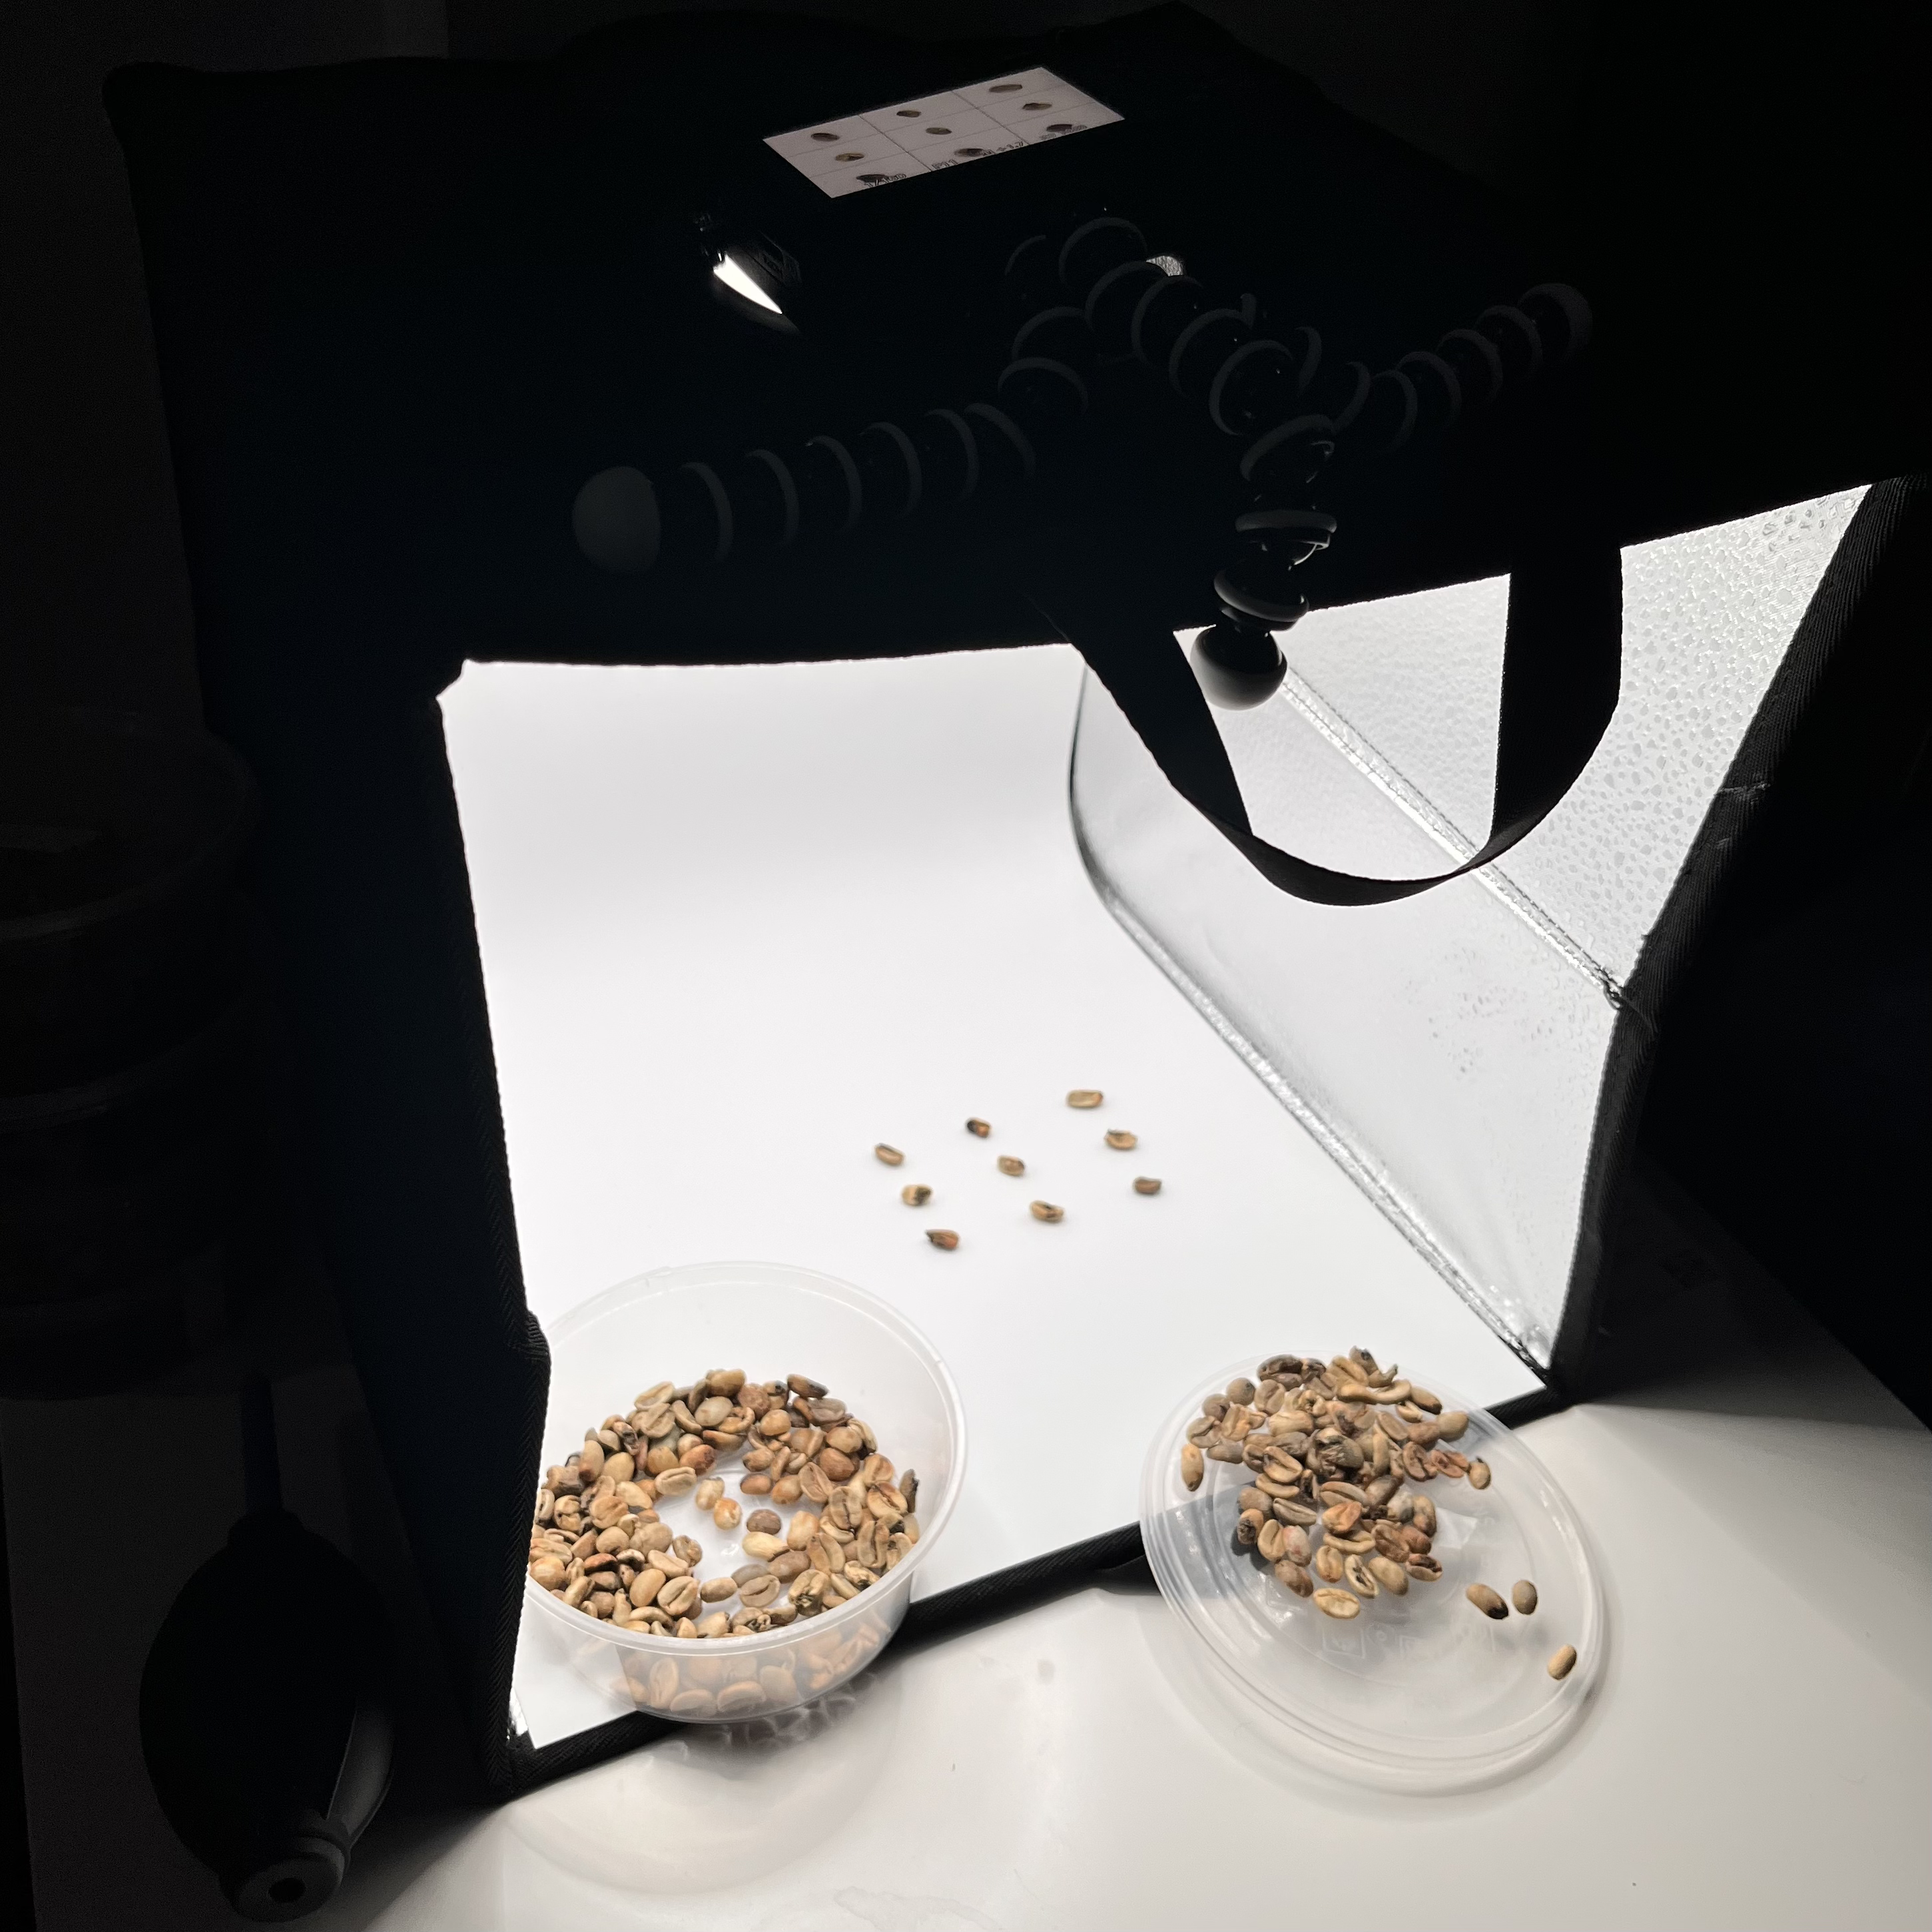
\includegraphics[width=6cm]{data_collection_setup.png}
    \caption{Data Collection Setup}
    \label{fig:data_collection_setup}
\end{figure}

% TODO: Table of Pics

The first iteration of data collection utilized a Sony A6300 camera with its Kit Lens, set at 1/200 Shutter Speed, 1000 ISO, and a Distance of 50mm. The beans were captured in batches of nine, carefully arranged within the camera's field of view following the rule of thirds. The rule of thirds is a photographic composition principle where an image is divided into a 3x3 grid, creating nine equal grid lines to create balance to the photo. By aligning the coffee beans with the rule of thirds, the group ensured a structured and even distribution of the beans within the frame. This setup also made it easier to automate the cropping process, as the predefined positions of the beans allowed a Python script to accurately extract individual images.

\subsection{2nd Iteration: Ideal Conditions}

% TODO: Table of Pics
The second iteration focused on real-world implementation, using the system's built-in webcam to capture images directly from the inspection tray. This setup represents the ideal condition, as it replicates the actual environment where the model will operate. The images captured in this iteration directly reflect what the system will process in a practical application, allowing for better generalization and real-time adaptability.

\section{Description of the System}

\begin{figure}[h]
    \centering
    \includegraphics[width=6cm]{ch5/system_block_diagram.png}
    \caption{System Block Diagram}
    \label{fig:system_block_diagram}
\end{figure}

The proposed system is a two-staged automated green coffeee bean sorting machine, integrating both machine vision and density analysis. Firstly, the coffee beans are introduced into the system through a funnel, which directs them to a conveyor belt mechanism.  In the first stage, the green coffee beans will be sorted depending on their visual characteristics. In this stage, the physical qualities of the bean is analyzed such as size, color, and defect. If the bean is defective, the system will automatically sort it out. Then, all the non-defective beans will go through the second stage of the system. In the second stage, there will be an IR sensor and a weighing scale. The IR sensor will help the system to calculate for the estimated volume of the bean. The volume and mass of the bean in hand, the density of the bean can be calculated. Depending on the density threshold and size threshold set by the user, the bean will be classified whether it is good or not.

\begin{figure}[h]
    \centering
    \includegraphics[width=6cm]{ch5/Schematic_Diagram_of_the_System.png}
    \caption{Schematic Diagram of the System}
    \label{fig:system_schematic_diagram}
\end{figure}

Figure \ref{fig:system_schematic_diagram} shows the schematic diagram of the proposed system. Arduino Uno microcontroller makes all the mechanical components such as the servo motor, stepper motors, and the conveyor belt. The servo motor controls the  rotating mechanism for bean sorting. On the other hand, the stepper motors operate a slide mechanism to direct the beans. Two cameras, integrated with OpenCV via Python, handle machine vision algorithms, and image processing for defect detection of the beans. A ToF10120 sensor provides precise distance measurement. A precision weighing scale measures the density of each bean for classification. The Arduino communicates with the OpenCV system through serial communication, ensuring smooth coordination.

\begin{figure}[h]
    \centering
    \includegraphics[width=6cm]{ch5/Overview_Of_The_System.png}
    \caption{Design Overview of the System}
    \label{fig:system_design_overview}
\end{figure}

Figure \ref{fig:system_design_overview} shows the design overview of the system. Beans are first arranged through a hopper and a conveyor belt. On top of the conveyor belt, a 3D-printed guide is attached for the beans to maintain a linear formation. Then, the beans are expected to fall into another funnel attached to a tube. The tube is directly attached to a rotating mechanism that allows the beans to be inspected and sorted one-by-one. In this stage, defective beans are sorted out. Then, the non-defective beans are transferred onto the precision scale to analyze the density. The less-dense beans are sorted out of the batch.

\section{Dataset and Model Training}
% TODO: Fix citations.
% ! REMOVE THE PARTS ABOUT RANDOM FOREST
For dataset collection, Arabica green beans from a farm will be used. Each bean will be captured by a high-resolution camera under sufficient and consistent lighting. Proper lighting is crucial, as it directly affects the visibility of the bean’s physical features, minimizing shadows, grain, and other noise that could result from inconsistent illumination. The top and bottom side pictures of the beans are to be collected. In addition, defective beans of the same type and origin will be gathered to identify the different classification of defects (primary and secondary). This study focuses on defects such as Broken, Dried Cherry, Floater, Full Black, Full Sour, Fungus Damage, and Insect Damage. The dataset will include at least 500 images of good beans and a minimum of 200 images for each defect category. To expand the dataset and enhance model training, augmentation techniques such as scaling, rotation, and mirroring will be applied.

The models to be used in this study are Convolutional Neural Network (CNN) and Random Forest. The CNN model is mostly compatible for image classification and feature extraction as it is composed of several different layers resulting in a better representation of image data (Wang et al., 2021). Thus, this model is the most ideal for green bean defect detection by identifying its texture, color, size, volume, deformations, and cracks in the first stage of sorting. Then, for the second stage where density parameter is added, Random Forest will be used. Since mixed data types are being considered (visual features extracted by CNN and density values), Random Forest is the best fit for this classification (Rigatti, 2017). In addition, the model is robust to overfitting, which means that it can handle noisy data. 

\section{Testing}
\label{sec:testing_and_evaluation}

For the testing procedures, processed but unsorted green coffee beans will be acquired from a local farmer. These coffee beans will be sorted manually based on their different defects and quality, and also will be fed into the automated system to compare accuracy and performance. In line with the Philippine National Standard  or PNS (2022) for testing green coffee bean sorters, three test trials will be conducted. These trials will be conducted under similar operational settinsg to ensure consistency. The duration of each trial begins when the beans are fed into the system’s hopper and endsd after no beans remain in the system. During these trials, the system’s ability to sort defective beans and categorize the good beans by density will be monitored.
To create the dataset, coffee beans will be arranged on a sheet of paper and photo of the entire sheet will be taken. A program using YOLOv8 will then be used to process this image, detecting each bean, creating bounding boxes, and crop them into separate image files for labeling. Additionally, an alternative method involves using the system itself to collect data, with cameras capturing the top and bottom of the beans as they pass through the system. These approaches aim to ensure to create a diverse dataset that will be used for training the machine learning model.

In evaluating the system’s performance, various metrics, as dictated by the PNS for Green Coffee Bean Sorters, will be considered: 
\begin{itemize}
	\item \textbf{Sorting Accuracy}. The system’s sorting accuracy will be verified by comparing the output of the system to the manually sorted output of the same batch of beans.
	\item \textbf{Duration of Tests}. The total operating time for each trial will be recorded.
	\item \textbf{Sorting Yield}. The quantity and quality of the beans sorted in each trial will be measured to assess the system.
\end{itemize}

	The desired accuracy of the system for its defect sorting is an accuracy of at least 85\%. The paper of Lualhati et al. (2022) was able to achieve an accuracy score of 85\% for sorting out good beans and 95\% for defect sorting, with an average score of 90\% for sorting out both. However, their paper only included two types of defects (black and deformed), and good quality beans as its data set. This study aims to target 10 types of defects along with the good green coffee beans ensuring that the system can cover a wider range of defects while also matching the accuracy of the previous study. 

	To validate the performance of the system, the results will be compared with those obtained during the manual sorting. This comparison will focus on determining the accuracy of the defect detection and bean classification. The manual sorting process will serve as the reference for evaluating the system’s ability to enhance sorting efficiency and accuracy.

% TODO: Following sections
\section{Data Analysis}
\section{System/Prototype Development} % Can be removed?
\section{Evaluation} % Can be removed/merged with `Testing`
\section{Summary}

Provide the gist of this chapter such that it reflects the contents and the message.
